\documentclass[1p]{elsarticle_modified}
%\bibliographystyle{elsarticle-num}

%\usepackage[colorlinks]{hyperref}
%\usepackage{abbrmath_seonhwa} %\Abb, \Ascr, \Acal ,\Abf, \Afrak
\usepackage{amsfonts}
\usepackage{amssymb}
\usepackage{amsmath}
\usepackage{amsthm}
\usepackage{scalefnt}
\usepackage{amsbsy}
\usepackage{kotex}
\usepackage{caption}
\usepackage{subfig}
\usepackage{color}
\usepackage{graphicx}
\usepackage{xcolor} %% white, black, red, green, blue, cyan, magenta, yellow
\usepackage{float}
\usepackage{setspace}
\usepackage{hyperref}

\usepackage{tikz}
\usetikzlibrary{arrows}

\usepackage{multirow}
\usepackage{array} % fixed length table
\usepackage{hhline}

%%%%%%%%%%%%%%%%%%%%%
\makeatletter
\renewcommand*\env@matrix[1][\arraystretch]{%
	\edef\arraystretch{#1}%
	\hskip -\arraycolsep
	\let\@ifnextchar\new@ifnextchar
	\array{*\c@MaxMatrixCols c}}
\makeatother %https://tex.stackexchange.com/questions/14071/how-can-i-increase-the-line-spacing-in-a-matrix
%%%%%%%%%%%%%%%

\usepackage[normalem]{ulem}

\newcommand{\msout}[1]{\ifmmode\text{\sout{\ensuremath{#1}}}\else\sout{#1}\fi}
%SOURCE: \msout is \stkout macro in https://tex.stackexchange.com/questions/20609/strikeout-in-math-mode

\newcommand{\cancel}[1]{
	\ifmmode
	{\color{red}\msout{#1}}
	\else
	{\color{red}\sout{#1}}
	\fi
}

\newcommand{\add}[1]{
	{\color{blue}\uwave{#1}}
}

\newcommand{\replace}[2]{
	\ifmmode
	{\color{red}\msout{#1}}{\color{blue}\uwave{#2}}
	\else
	{\color{red}\sout{#1}}{\color{blue}\uwave{#2}}
	\fi
}

\newcommand{\Sol}{\mathcal{S}} %segment
\newcommand{\D}{D} %diagram
\newcommand{\A}{\mathcal{A}} %arc


%%%%%%%%%%%%%%%%%%%%%%%%%%%%%5 test

\def\sl{\operatorname{\textup{SL}}(2,\Cbb)}
\def\psl{\operatorname{\textup{PSL}}(2,\Cbb)}
\def\quan{\mkern 1mu \triangleright \mkern 1mu}

\theoremstyle{definition}
\newtheorem{thm}{Theorem}[section]
\newtheorem{prop}[thm]{Proposition}
\newtheorem{lem}[thm]{Lemma}
\newtheorem{ques}[thm]{Question}
\newtheorem{cor}[thm]{Corollary}
\newtheorem{defn}[thm]{Definition}
\newtheorem{exam}[thm]{Example}
\newtheorem{rmk}[thm]{Remark}
\newtheorem{alg}[thm]{Algorithm}

\newcommand{\I}{\sqrt{-1}}
\begin{document}

%\begin{frontmatter}
%
%\title{Boundary parabolic representations of knots up to 8 crossings}
%
%%% Group authors per affiliation:
%\author{Yunhi Cho} 
%\address{Department of Mathematics, University of Seoul, Seoul, Korea}
%\ead{yhcho@uos.ac.kr}
%
%
%\author{Seonhwa Kim} %\fnref{s_kim}}
%\address{Center for Geometry and Physics, Institute for Basic Science, Pohang, 37673, Korea}
%\ead{ryeona17@ibs.re.kr}
%
%\author{Hyuk Kim}
%\address{Department of Mathematical Sciences, Seoul National University, Seoul 08826, Korea}
%\ead{hyukkim@snu.ac.kr}
%
%\author{Seokbeom Yoon}
%\address{Department of Mathematical Sciences, Seoul National University, Seoul, 08826,  Korea}
%\ead{sbyoon15@snu.ac.kr}
%
%\begin{abstract}
%We find all boundary parabolic representation of knots up to 8 crossings.
%
%\end{abstract}
%\begin{keyword}
%    \MSC[2010] 57M25 
%\end{keyword}
%
%\end{frontmatter}

%\linenumbers
%\tableofcontents
%
\newcommand\colored[1]{\textcolor{white}{\rule[-0.35ex]{0.8em}{1.4ex}}\kern-0.8em\color{red} #1}%
%\newcommand\colored[1]{\textcolor{white}{ #1}\kern-2.17ex	\textcolor{white}{ #1}\kern-1.81ex	\textcolor{white}{ #1}\kern-2.15ex\color{red}#1	}

{\Large $\underline{12a_{0170}~(K12a_{0170})}$}

\setlength{\tabcolsep}{10pt}
\renewcommand{\arraystretch}{1.6}
\vspace{1cm}\begin{tabular}{m{100pt}>{\centering\arraybackslash}m{274pt}}
\multirow{5}{120pt}{
	\centering
	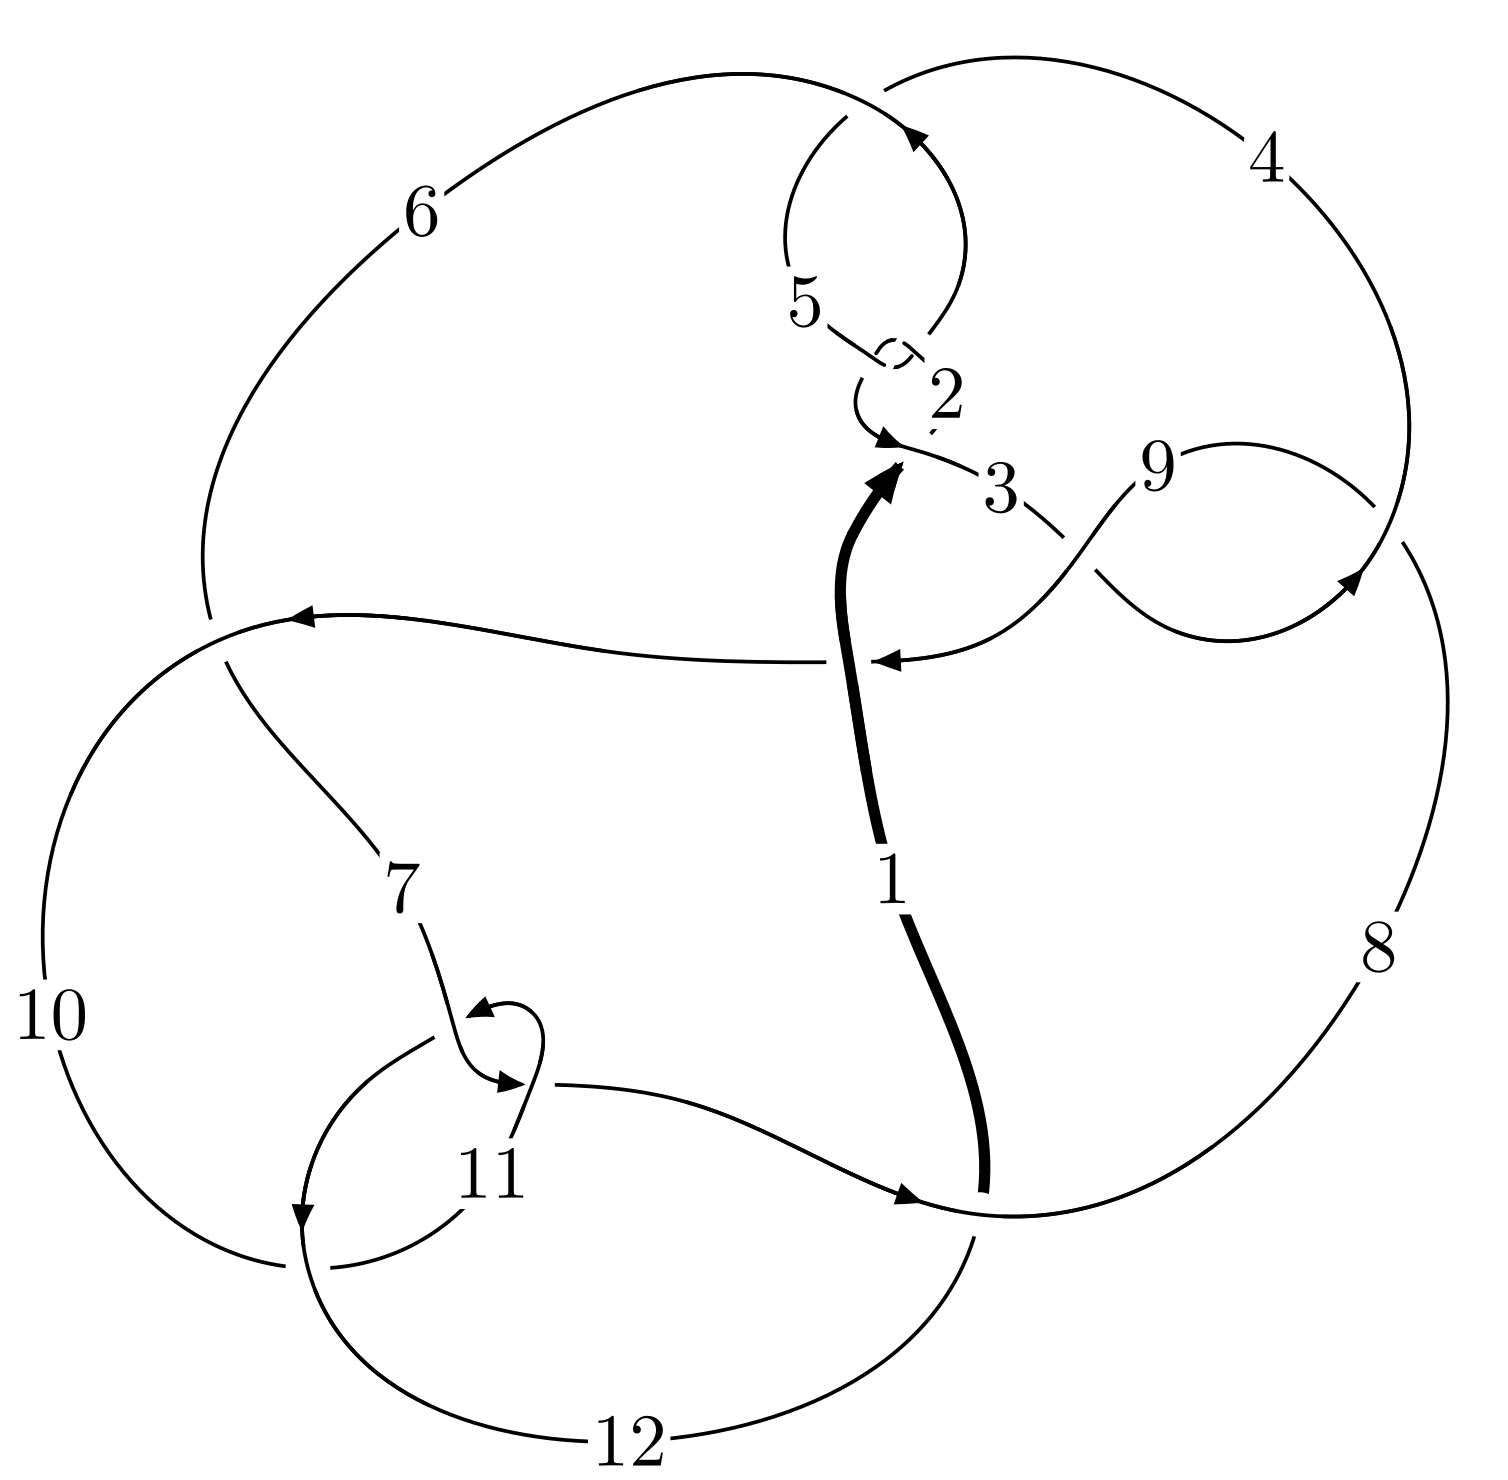
\includegraphics[width=112pt]{../../../GIT/diagram.site/Diagrams/png/971_12a_0170.png}\\
\ \ \ A knot diagram\footnotemark}&
\allowdisplaybreaks
\textbf{Linearized knot diagam} \\
\cline{2-2}
 &
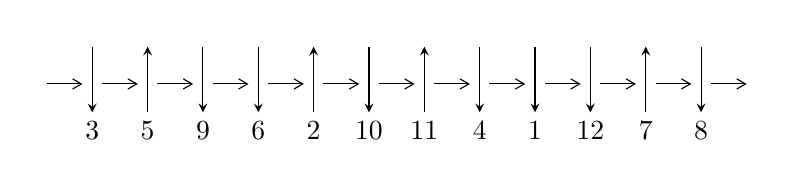
\begin{tikzpicture}[x=20pt, y=17pt]
	% nodes
	\node (C0) at (0, 0) {};
	\node (C1) at (1, 0) {};
	\node (C1U) at (1, +1) {};
	\node (C1D) at (1, -1) {3};

	\node (C2) at (2, 0) {};
	\node (C2U) at (2, +1) {};
	\node (C2D) at (2, -1) {5};

	\node (C3) at (3, 0) {};
	\node (C3U) at (3, +1) {};
	\node (C3D) at (3, -1) {9};

	\node (C4) at (4, 0) {};
	\node (C4U) at (4, +1) {};
	\node (C4D) at (4, -1) {6};

	\node (C5) at (5, 0) {};
	\node (C5U) at (5, +1) {};
	\node (C5D) at (5, -1) {2};

	\node (C6) at (6, 0) {};
	\node (C6U) at (6, +1) {};
	\node (C6D) at (6, -1) {10};

	\node (C7) at (7, 0) {};
	\node (C7U) at (7, +1) {};
	\node (C7D) at (7, -1) {11};

	\node (C8) at (8, 0) {};
	\node (C8U) at (8, +1) {};
	\node (C8D) at (8, -1) {4};

	\node (C9) at (9, 0) {};
	\node (C9U) at (9, +1) {};
	\node (C9D) at (9, -1) {1};

	\node (C10) at (10, 0) {};
	\node (C10U) at (10, +1) {};
	\node (C10D) at (10, -1) {12};

	\node (C11) at (11, 0) {};
	\node (C11U) at (11, +1) {};
	\node (C11D) at (11, -1) {7};

	\node (C12) at (12, 0) {};
	\node (C12U) at (12, +1) {};
	\node (C12D) at (12, -1) {8};
	\node (C13) at (13, 0) {};

	% arrows
	\draw[->,>={angle 60}]
	(C0) edge (C1) (C1) edge (C2) (C2) edge (C3) (C3) edge (C4) (C4) edge (C5) (C5) edge (C6) (C6) edge (C7) (C7) edge (C8) (C8) edge (C9) (C9) edge (C10) (C10) edge (C11) (C11) edge (C12) (C12) edge (C13) ;	\draw[->,>=stealth]
	(C1U) edge (C1D) (C2D) edge (C2U) (C3U) edge (C3D) (C4U) edge (C4D) (C5D) edge (C5U) (C6U) edge (C6D) (C7D) edge (C7U) (C8U) edge (C8D) (C9U) edge (C9D) (C10U) edge (C10D) (C11D) edge (C11U) (C12U) edge (C12D) ;
	\end{tikzpicture} \\
\hhline{~~} \\& 
\textbf{Solving Sequence} \\ \cline{2-2} 
 &
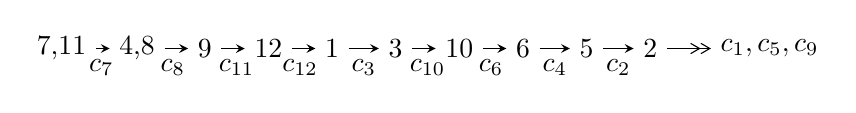
\begin{tikzpicture}[x=23pt, y=7pt]
	% node
	\node (A0) at (-1/8, 0) {7,11};
	\node (A1) at (17/16, 0) {4,8};
	\node (A2) at (17/8, 0) {9};
	\node (A3) at (25/8, 0) {12};
	\node (A4) at (33/8, 0) {1};
	\node (A5) at (41/8, 0) {3};
	\node (A6) at (49/8, 0) {10};
	\node (A7) at (57/8, 0) {6};
	\node (A8) at (65/8, 0) {5};
	\node (A9) at (73/8, 0) {2};
	\node (C1) at (1/2, -1) {$c_{7}$};
	\node (C2) at (13/8, -1) {$c_{8}$};
	\node (C3) at (21/8, -1) {$c_{11}$};
	\node (C4) at (29/8, -1) {$c_{12}$};
	\node (C5) at (37/8, -1) {$c_{3}$};
	\node (C6) at (45/8, -1) {$c_{10}$};
	\node (C7) at (53/8, -1) {$c_{6}$};
	\node (C8) at (61/8, -1) {$c_{4}$};
	\node (C9) at (69/8, -1) {$c_{2}$};
	\node (A10) at (11, 0) {$c_{1},c_{5},c_{9}$};

	% edge
	\draw[->,>=stealth]	
	(A0) edge (A1) (A1) edge (A2) (A2) edge (A3) (A3) edge (A4) (A4) edge (A5) (A5) edge (A6) (A6) edge (A7) (A7) edge (A8) (A8) edge (A9) ;
	\draw[->>,>={angle 60}]	
	(A9) edge (A10);
\end{tikzpicture} \\ 

\end{tabular} \\

\footnotetext{
The image of knot diagram is generated by the software ``\textbf{Draw programme}" developed by Andrew Bartholomew(\url{http://www.layer8.co.uk/maths/draw/index.htm\#Running-draw}), where we modified some parts for our purpose(\url{https://github.com/CATsTAILs/LinksPainter}).
}\phantom \\ \newline 
\centering \textbf{Ideals for irreducible components\footnotemark of $X_{\text{par}}$} 
 
\begin{align*}
I^u_{1}&=\langle 
8 u^{98}+22 u^{97}+\cdots+2 b-8 u,\;8 u^{98}+24 u^{97}+\cdots+2 a-11,\;u^{99}+3 u^{98}+\cdots-5 u-1\rangle \\
I^u_{2}&=\langle 
u^2 a+b,\;u^4+u^2 a-2 u^3+a^2- a u+3 u^2+a-2 u+1,\;u^5- u^4+2 u^3- u^2+u-1\rangle \\
\\
\end{align*}
\raggedright * 2 irreducible components of $\dim_{\mathbb{C}}=0$, with total 109 representations.\\
\footnotetext{All coefficients of polynomials are rational numbers. But the coefficients are sometimes approximated in decimal forms when there is not enough margin.}
\newpage
\renewcommand{\arraystretch}{1}
\centering \section*{I. $I^u_{1}= \langle 8 u^{98}+22 u^{97}+\cdots+2 b-8 u,\;8 u^{98}+24 u^{97}+\cdots+2 a-11,\;u^{99}+3 u^{98}+\cdots-5 u-1 \rangle$}
\flushleft \textbf{(i) Arc colorings}\\
\begin{tabular}{m{7pt} m{180pt} m{7pt} m{180pt} }
\flushright $a_{7}=$&$\begin{pmatrix}1\\0\end{pmatrix}$ \\
\flushright $a_{11}=$&$\begin{pmatrix}0\\u\end{pmatrix}$ \\
\flushright $a_{4}=$&$\begin{pmatrix}-4 u^{98}-12 u^{97}+\cdots+27 u+\frac{11}{2}\\-4 u^{98}-11 u^{97}+\cdots+\frac{19}{2} u^2+4 u\end{pmatrix}$ \\
\flushright $a_{8}=$&$\begin{pmatrix}1\\- u^2\end{pmatrix}$ \\
\flushright $a_{9}=$&$\begin{pmatrix}u^{11}+2 u^9+2 u^7+u^3\\- u^{13}-3 u^{11}-5 u^9-4 u^7-2 u^5+u^3+u\end{pmatrix}$ \\
\flushright $a_{12}=$&$\begin{pmatrix}u\\u\end{pmatrix}$ \\
\flushright $a_{1}=$&$\begin{pmatrix}- u^3\\u^5+u^3+u\end{pmatrix}$ \\
\flushright $a_{3}=$&$\begin{pmatrix}4 u^{97}+8 u^{96}+\cdots-11 u^2-\frac{1}{2}\\2 u^{97}+\frac{7}{2} u^{96}+\cdots-\frac{25}{2} u^2-2 u\end{pmatrix}$ \\
\flushright $a_{10}=$&$\begin{pmatrix}u^3\\u^3+u\end{pmatrix}$ \\
\flushright $a_{6}=$&$\begin{pmatrix}- u^6- u^4+1\\- u^6-2 u^4- u^2\end{pmatrix}$ \\
\flushright $a_{5}=$&$\begin{pmatrix}-2 u^{98}-\frac{9}{2} u^{97}+\cdots+13 u+2\\-2 u^{98}-\frac{9}{2} u^{97}+\cdots-2 u^2+\frac{1}{2} u\end{pmatrix}$ \\
\flushright $a_{2}=$&$\begin{pmatrix}-\frac{1}{2} u^{94}- u^{93}+\cdots+2 u-\frac{1}{2}\\\frac{1}{2} u^{96}+u^{95}+\cdots+\frac{3}{2} u^2+2 u\end{pmatrix}$\\&\end{tabular}
\flushleft \textbf{(ii) Obstruction class $= -1$}\\~\\
\flushleft \textbf{(iii) Cusp Shapes $= -4 u^{98}-\frac{41}{2} u^{97}+\cdots+55 u+\frac{15}{2}$}\\~\\
\newpage\renewcommand{\arraystretch}{1}
\flushleft \textbf{(iv) u-Polynomials at the component}\newline \\
\begin{tabular}{m{50pt}|m{274pt}}
Crossings & \hspace{64pt}u-Polynomials at each crossing \\
\hline $$\begin{aligned}c_{1},c_{4}\end{aligned}$$&$\begin{aligned}
&u^{99}+32 u^{98}+\cdots-28 u-1
\end{aligned}$\\
\hline $$\begin{aligned}c_{2},c_{5}\end{aligned}$$&$\begin{aligned}
&u^{99}+6 u^{98}+\cdots+4 u+1
\end{aligned}$\\
\hline $$\begin{aligned}c_{3},c_{8}\end{aligned}$$&$\begin{aligned}
&u^{99}+u^{98}+\cdots+3072 u+1024
\end{aligned}$\\
\hline $$\begin{aligned}c_{6},c_{12}\end{aligned}$$&$\begin{aligned}
&u^{99}+3 u^{98}+\cdots+1403 u+73
\end{aligned}$\\
\hline $$\begin{aligned}c_{7},c_{11}\end{aligned}$$&$\begin{aligned}
&u^{99}-3 u^{98}+\cdots-5 u+1
\end{aligned}$\\
\hline $$\begin{aligned}c_{9}\end{aligned}$$&$\begin{aligned}
&u^{99}-11 u^{98}+\cdots+27259 u+3341
\end{aligned}$\\
\hline $$\begin{aligned}c_{10}\end{aligned}$$&$\begin{aligned}
&u^{99}+53 u^{98}+\cdots-13 u-1
\end{aligned}$\\
\hline
\end{tabular}\\~\\
\newpage\renewcommand{\arraystretch}{1}
\flushleft \textbf{(v) Riley Polynomials at the component}\newline \\
\begin{tabular}{m{50pt}|m{274pt}}
Crossings & \hspace{64pt}Riley Polynomials at each crossing \\
\hline $$\begin{aligned}c_{1},c_{4}\end{aligned}$$&$\begin{aligned}
&y^{99}+76 y^{98}+\cdots+624 y-1
\end{aligned}$\\
\hline $$\begin{aligned}c_{2},c_{5}\end{aligned}$$&$\begin{aligned}
&y^{99}+32 y^{98}+\cdots-28 y-1
\end{aligned}$\\
\hline $$\begin{aligned}c_{3},c_{8}\end{aligned}$$&$\begin{aligned}
&y^{99}+55 y^{98}+\cdots-17825792 y-1048576
\end{aligned}$\\
\hline $$\begin{aligned}c_{6},c_{12}\end{aligned}$$&$\begin{aligned}
&y^{99}-75 y^{98}+\cdots+237579 y-5329
\end{aligned}$\\
\hline $$\begin{aligned}c_{7},c_{11}\end{aligned}$$&$\begin{aligned}
&y^{99}+53 y^{98}+\cdots-13 y-1
\end{aligned}$\\
\hline $$\begin{aligned}c_{9}\end{aligned}$$&$\begin{aligned}
&y^{99}+25 y^{98}+\cdots-762194377 y-11162281
\end{aligned}$\\
\hline $$\begin{aligned}c_{10}\end{aligned}$$&$\begin{aligned}
&y^{99}-11 y^{98}+\cdots+27 y-1
\end{aligned}$\\
\hline
\end{tabular}\\~\\
\newpage\flushleft \textbf{(vi) Complex Volumes and Cusp Shapes}
$$\begin{array}{c|c|c}  
\text{Solutions to }I^u_{1}& \I (\text{vol} + \sqrt{-1}CS) & \text{Cusp shape}\\
 \hline 
\begin{aligned}
u &= -0.429848 + 0.885673 I \\
a &= -0.153546 - 0.767268 I \\
b &= -0.0361333 - 0.0736755 I\end{aligned}
 & -1.19873 - 2.05854 I & \phantom{-0.000000 } 0 \\ \hline\begin{aligned}
u &= -0.429848 - 0.885673 I \\
a &= -0.153546 + 0.767268 I \\
b &= -0.0361333 + 0.0736755 I\end{aligned}
 & -1.19873 + 2.05854 I & \phantom{-0.000000 } 0 \\ \hline\begin{aligned}
u &= \phantom{-}0.520030 + 0.825601 I \\
a &= \phantom{-}1.59459 + 1.62990 I \\
b &= \phantom{-}1.73104 + 0.30568 I\end{aligned}
 & \phantom{-}0.30032 + 5.50967 I & \phantom{-0.000000 } 0 \\ \hline\begin{aligned}
u &= \phantom{-}0.520030 - 0.825601 I \\
a &= \phantom{-}1.59459 - 1.62990 I \\
b &= \phantom{-}1.73104 - 0.30568 I\end{aligned}
 & \phantom{-}0.30032 - 5.50967 I & \phantom{-0.000000 } 0 \\ \hline\begin{aligned}
u &= -0.067585 + 0.970965 I \\
a &= \phantom{-}1.71635 + 0.65270 I \\
b &= \phantom{-}0.985452 + 0.092942 I\end{aligned}
 & -3.46773 - 2.14043 I & \phantom{-0.000000 } 0 \\ \hline\begin{aligned}
u &= -0.067585 - 0.970965 I \\
a &= \phantom{-}1.71635 - 0.65270 I \\
b &= \phantom{-}0.985452 - 0.092942 I\end{aligned}
 & -3.46773 + 2.14043 I & \phantom{-0.000000 } 0 \\ \hline\begin{aligned}
u &= \phantom{-}0.589960 + 0.841124 I \\
a &= -1.72526 - 1.03952 I \\
b &= -1.192410 - 0.035831 I\end{aligned}
 & \phantom{-}7.81127 + 4.92186 I & \phantom{-0.000000 } 0 \\ \hline\begin{aligned}
u &= \phantom{-}0.589960 - 0.841124 I \\
a &= -1.72526 + 1.03952 I \\
b &= -1.192410 + 0.035831 I\end{aligned}
 & \phantom{-}7.81127 - 4.92186 I & \phantom{-0.000000 } 0 \\ \hline\begin{aligned}
u &= \phantom{-}0.587785 + 0.858222 I \\
a &= \phantom{-}1.85438 + 1.06685 I \\
b &= \phantom{-}1.239810 - 0.106984 I\end{aligned}
 & \phantom{-}6.97384 + 11.00210 I & \phantom{-0.000000 } 0 \\ \hline\begin{aligned}
u &= \phantom{-}0.587785 - 0.858222 I \\
a &= \phantom{-}1.85438 - 1.06685 I \\
b &= \phantom{-}1.239810 + 0.106984 I\end{aligned}
 & \phantom{-}6.97384 - 11.00210 I & \phantom{-0.000000 } 0\\
 \hline 
 \end{array}$$\newpage$$\begin{array}{c|c|c}  
\text{Solutions to }I^u_{1}& \I (\text{vol} + \sqrt{-1}CS) & \text{Cusp shape}\\
 \hline 
\begin{aligned}
u &= -0.539698 + 0.786920 I \\
a &= \phantom{-}0.322917 - 1.006990 I \\
b &= -0.159118 + 0.087102 I\end{aligned}
 & \phantom{-}3.08688 - 4.97900 I & \phantom{-0.000000 } 0 \\ \hline\begin{aligned}
u &= -0.539698 - 0.786920 I \\
a &= \phantom{-}0.322917 + 1.006990 I \\
b &= -0.159118 - 0.087102 I\end{aligned}
 & \phantom{-}3.08688 + 4.97900 I & \phantom{-0.000000 } 0 \\ \hline\begin{aligned}
u &= \phantom{-}0.547960 + 0.768863 I \\
a &= -1.07630 - 1.33495 I \\
b &= -1.38296 - 0.64272 I\end{aligned}
 & \phantom{-}3.91657 + 2.20363 I & \phantom{-0.000000 } 0 \\ \hline\begin{aligned}
u &= \phantom{-}0.547960 - 0.768863 I \\
a &= -1.07630 + 1.33495 I \\
b &= -1.38296 + 0.64272 I\end{aligned}
 & \phantom{-}3.91657 - 2.20363 I & \phantom{-0.000000 } 0 \\ \hline\begin{aligned}
u &= -0.537978 + 0.751303 I \\
a &= -0.405247 + 0.942552 I \\
b &= \phantom{-}0.237597 - 0.042309 I\end{aligned}
 & \phantom{-}3.19000 + 0.62409 I & \phantom{-0.000000 } 0 \\ \hline\begin{aligned}
u &= -0.537978 - 0.751303 I \\
a &= -0.405247 - 0.942552 I \\
b &= \phantom{-}0.237597 + 0.042309 I\end{aligned}
 & \phantom{-}3.19000 - 0.62409 I & \phantom{-0.000000 } 0 \\ \hline\begin{aligned}
u &= \phantom{-}0.610078 + 0.689564 I \\
a &= -0.538676 - 0.708628 I \\
b &= -1.03942 - 1.00260 I\end{aligned}
 & \phantom{-}8.24446 - 0.21969 I & \phantom{-0.000000 } 0 \\ \hline\begin{aligned}
u &= \phantom{-}0.610078 - 0.689564 I \\
a &= -0.538676 + 0.708628 I \\
b &= -1.03942 + 1.00260 I\end{aligned}
 & \phantom{-}8.24446 + 0.21969 I & \phantom{-0.000000 } 0 \\ \hline\begin{aligned}
u &= \phantom{-}0.613989 + 0.666989 I \\
a &= \phantom{-}0.385176 + 0.652596 I \\
b &= \phantom{-}1.05850 + 1.08315 I\end{aligned}
 & \phantom{-}7.51964 - 6.29705 I & \phantom{-0.000000 } 0 \\ \hline\begin{aligned}
u &= \phantom{-}0.613989 - 0.666989 I \\
a &= \phantom{-}0.385176 - 0.652596 I \\
b &= \phantom{-}1.05850 - 1.08315 I\end{aligned}
 & \phantom{-}7.51964 + 6.29705 I & \phantom{-0.000000 } 0\\
 \hline 
 \end{array}$$\newpage$$\begin{array}{c|c|c}  
\text{Solutions to }I^u_{1}& \I (\text{vol} + \sqrt{-1}CS) & \text{Cusp shape}\\
 \hline 
\begin{aligned}
u &= -0.148795 + 1.100110 I \\
a &= \phantom{-}1.30891 + 1.51158 I \\
b &= \phantom{-}0.641318 + 1.037130 I\end{aligned}
 & \phantom{-}1.74742 - 6.77346 I & \phantom{-0.000000 } 0 \\ \hline\begin{aligned}
u &= -0.148795 - 1.100110 I \\
a &= \phantom{-}1.30891 - 1.51158 I \\
b &= \phantom{-}0.641318 - 1.037130 I\end{aligned}
 & \phantom{-}1.74742 + 6.77346 I & \phantom{-0.000000 } 0 \\ \hline\begin{aligned}
u &= -0.186308 + 1.098120 I \\
a &= -1.03578 - 1.47748 I \\
b &= -0.333673 - 0.963763 I\end{aligned}
 & \phantom{-}2.34741 - 1.01757 I & \phantom{-0.000000 } 0 \\ \hline\begin{aligned}
u &= -0.186308 - 1.098120 I \\
a &= -1.03578 + 1.47748 I \\
b &= -0.333673 + 0.963763 I\end{aligned}
 & \phantom{-}2.34741 + 1.01757 I & \phantom{-0.000000 } 0 \\ \hline\begin{aligned}
u &= \phantom{-}0.498411 + 0.706670 I \\
a &= \phantom{-}0.38383 + 1.60293 I \\
b &= \phantom{-}1.42427 + 1.06732 I\end{aligned}
 & \phantom{-}0.65077 - 1.31271 I & -0.53545 + 1.30950 I \\ \hline\begin{aligned}
u &= \phantom{-}0.498411 - 0.706670 I \\
a &= \phantom{-}0.38383 - 1.60293 I \\
b &= \phantom{-}1.42427 - 1.06732 I\end{aligned}
 & \phantom{-}0.65077 + 1.31271 I & -0.53545 - 1.30950 I \\ \hline\begin{aligned}
u &= -0.820785 + 0.171758 I \\
a &= \phantom{-}1.304340 + 0.375554 I \\
b &= -1.60855 + 1.40861 I\end{aligned}
 & \phantom{-}3.47980 + 11.99530 I & -1.53503 - 7.47840 I \\ \hline\begin{aligned}
u &= -0.820785 - 0.171758 I \\
a &= \phantom{-}1.304340 - 0.375554 I \\
b &= -1.60855 - 1.40861 I\end{aligned}
 & \phantom{-}3.47980 - 11.99530 I & -1.53503 + 7.47840 I \\ \hline\begin{aligned}
u &= \phantom{-}0.833946 + 0.012856 I \\
a &= \phantom{-}0.084871 - 0.732326 I \\
b &= -0.19316 + 1.42037 I\end{aligned}
 & -1.20309 + 2.61578 I & -0.20305 - 3.89462 I \\ \hline\begin{aligned}
u &= \phantom{-}0.833946 - 0.012856 I \\
a &= \phantom{-}0.084871 + 0.732326 I \\
b &= -0.19316 - 1.42037 I\end{aligned}
 & -1.20309 - 2.61578 I & -0.20305 + 3.89462 I\\
 \hline 
 \end{array}$$\newpage$$\begin{array}{c|c|c}  
\text{Solutions to }I^u_{1}& \I (\text{vol} + \sqrt{-1}CS) & \text{Cusp shape}\\
 \hline 
\begin{aligned}
u &= -0.810571 + 0.181206 I \\
a &= -1.195870 - 0.405767 I \\
b &= \phantom{-}1.44493 - 1.40454 I\end{aligned}
 & \phantom{-}4.51727 + 5.99226 I & \phantom{-}0.25329 - 2.79129 I \\ \hline\begin{aligned}
u &= -0.810571 - 0.181206 I \\
a &= -1.195870 + 0.405767 I \\
b &= \phantom{-}1.44493 + 1.40454 I\end{aligned}
 & \phantom{-}4.51727 - 5.99226 I & \phantom{-}0.25329 + 2.79129 I \\ \hline\begin{aligned}
u &= \phantom{-}0.116457 + 0.819121 I \\
a &= \phantom{-}2.36072 - 0.47151 I \\
b &= \phantom{-}0.92714 - 1.16497 I\end{aligned}
 & -0.91323 + 2.95442 I & -9.15892 - 0.78061 I \\ \hline\begin{aligned}
u &= \phantom{-}0.116457 - 0.819121 I \\
a &= \phantom{-}2.36072 + 0.47151 I \\
b &= \phantom{-}0.92714 + 1.16497 I\end{aligned}
 & -0.91323 - 2.95442 I & -9.15892 + 0.78061 I \\ \hline\begin{aligned}
u &= -0.278900 + 0.753215 I \\
a &= -0.665243 + 0.280196 I \\
b &= -0.087537 + 0.193088 I\end{aligned}
 & -0.383982 - 1.218840 I & -4.66040 + 5.43923 I \\ \hline\begin{aligned}
u &= -0.278900 - 0.753215 I \\
a &= -0.665243 - 0.280196 I \\
b &= -0.087537 - 0.193088 I\end{aligned}
 & -0.383982 + 1.218840 I & -4.66040 - 5.43923 I \\ \hline\begin{aligned}
u &= -0.521477 + 1.085120 I \\
a &= -1.18894 - 0.85234 I \\
b &= -0.378212 - 0.754350 I\end{aligned}
 & \phantom{-}4.02781 - 0.01979 I & \phantom{-0.000000 } 0 \\ \hline\begin{aligned}
u &= -0.521477 - 1.085120 I \\
a &= -1.18894 + 0.85234 I \\
b &= -0.378212 + 0.754350 I\end{aligned}
 & \phantom{-}4.02781 + 0.01979 I & \phantom{-0.000000 } 0 \\ \hline\begin{aligned}
u &= -0.780382 + 0.143990 I \\
a &= \phantom{-}1.30030 + 0.80184 I \\
b &= -1.44582 + 0.86730 I\end{aligned}
 & -2.65965 + 5.88729 I & -5.59627 - 5.93514 I \\ \hline\begin{aligned}
u &= -0.780382 - 0.143990 I \\
a &= \phantom{-}1.30030 - 0.80184 I \\
b &= -1.44582 - 0.86730 I\end{aligned}
 & -2.65965 - 5.88729 I & -5.59627 + 5.93514 I\\
 \hline 
 \end{array}$$\newpage$$\begin{array}{c|c|c}  
\text{Solutions to }I^u_{1}& \I (\text{vol} + \sqrt{-1}CS) & \text{Cusp shape}\\
 \hline 
\begin{aligned}
u &= \phantom{-}0.782638 + 0.077219 I \\
a &= \phantom{-}0.512667 - 0.508839 I \\
b &= -1.042870 + 0.788319 I\end{aligned}
 & -4.26717 - 1.31247 I & -9.29800 + 0.03301 I \\ \hline\begin{aligned}
u &= \phantom{-}0.782638 - 0.077219 I \\
a &= \phantom{-}0.512667 + 0.508839 I \\
b &= -1.042870 - 0.788319 I\end{aligned}
 & -4.26717 + 1.31247 I & -9.29800 - 0.03301 I \\ \hline\begin{aligned}
u &= \phantom{-}0.387534 + 1.152560 I \\
a &= \phantom{-}2.31597 + 0.24090 I \\
b &= \phantom{-}1.94984 - 1.44963 I\end{aligned}
 & -2.70236 + 3.53975 I & \phantom{-0.000000 } 0 \\ \hline\begin{aligned}
u &= \phantom{-}0.387534 - 1.152560 I \\
a &= \phantom{-}2.31597 - 0.24090 I \\
b &= \phantom{-}1.94984 + 1.44963 I\end{aligned}
 & -2.70236 - 3.53975 I & \phantom{-0.000000 } 0 \\ \hline\begin{aligned}
u &= -0.374340 + 1.157870 I \\
a &= \phantom{-}0.439971 - 0.718676 I \\
b &= \phantom{-}0.791182 + 0.555743 I\end{aligned}
 & -2.30156 - 0.62216 I & \phantom{-0.000000 } 0 \\ \hline\begin{aligned}
u &= -0.374340 - 1.157870 I \\
a &= \phantom{-}0.439971 + 0.718676 I \\
b &= \phantom{-}0.791182 - 0.555743 I\end{aligned}
 & -2.30156 + 0.62216 I & \phantom{-0.000000 } 0 \\ \hline\begin{aligned}
u &= -0.524450 + 1.104260 I \\
a &= \phantom{-}1.39278 + 0.74600 I \\
b &= \phantom{-}0.598909 + 0.920885 I\end{aligned}
 & \phantom{-}4.36503 - 6.08039 I & \phantom{-0.000000 } 0 \\ \hline\begin{aligned}
u &= -0.524450 - 1.104260 I \\
a &= \phantom{-}1.39278 - 0.74600 I \\
b &= \phantom{-}0.598909 - 0.920885 I\end{aligned}
 & \phantom{-}4.36503 + 6.08039 I & \phantom{-0.000000 } 0 \\ \hline\begin{aligned}
u &= \phantom{-}0.754778 + 0.164359 I \\
a &= \phantom{-}0.809503 - 0.494638 I \\
b &= -1.66362 + 0.41793 I\end{aligned}
 & \phantom{-}0.49832 - 5.62398 I & -2.47133 + 4.97773 I \\ \hline\begin{aligned}
u &= \phantom{-}0.754778 - 0.164359 I \\
a &= \phantom{-}0.809503 + 0.494638 I \\
b &= -1.66362 - 0.41793 I\end{aligned}
 & \phantom{-}0.49832 + 5.62398 I & -2.47133 - 4.97773 I\\
 \hline 
 \end{array}$$\newpage$$\begin{array}{c|c|c}  
\text{Solutions to }I^u_{1}& \I (\text{vol} + \sqrt{-1}CS) & \text{Cusp shape}\\
 \hline 
\begin{aligned}
u &= \phantom{-}0.374341 + 1.174030 I \\
a &= -2.42621 + 0.01899 I \\
b &= -1.94987 + 1.72785 I\end{aligned}
 & -3.38821 - 1.91522 I & \phantom{-0.000000 } 0 \\ \hline\begin{aligned}
u &= \phantom{-}0.374341 - 1.174030 I \\
a &= -2.42621 - 0.01899 I \\
b &= -1.94987 - 1.72785 I\end{aligned}
 & -3.38821 + 1.91522 I & \phantom{-0.000000 } 0 \\ \hline\begin{aligned}
u &= -0.698389 + 0.314322 I \\
a &= -0.145640 - 0.527804 I \\
b &= \phantom{-}0.057658 - 1.217660 I\end{aligned}
 & \phantom{-}6.65889 + 1.40997 I & \phantom{-}2.43753 - 1.73189 I \\ \hline\begin{aligned}
u &= -0.698389 - 0.314322 I \\
a &= -0.145640 + 0.527804 I \\
b &= \phantom{-}0.057658 + 1.217660 I\end{aligned}
 & \phantom{-}6.65889 - 1.40997 I & \phantom{-}2.43753 + 1.73189 I \\ \hline\begin{aligned}
u &= -0.411903 + 1.165120 I \\
a &= -0.540539 - 0.017453 I \\
b &= -0.29700 - 1.42113 I\end{aligned}
 & -4.64701 - 4.92563 I & \phantom{-0.000000 } 0 \\ \hline\begin{aligned}
u &= -0.411903 - 1.165120 I \\
a &= -0.540539 + 0.017453 I \\
b &= -0.29700 + 1.42113 I\end{aligned}
 & -4.64701 + 4.92563 I & \phantom{-0.000000 } 0 \\ \hline\begin{aligned}
u &= -0.682190 + 0.343573 I \\
a &= \phantom{-}0.007635 + 0.534085 I \\
b &= \phantom{-}0.102783 + 1.150590 I\end{aligned}
 & \phantom{-}6.17569 - 4.60385 I & \phantom{-}1.65384 + 3.69650 I \\ \hline\begin{aligned}
u &= -0.682190 - 0.343573 I \\
a &= \phantom{-}0.007635 - 0.534085 I \\
b &= \phantom{-}0.102783 - 1.150590 I\end{aligned}
 & \phantom{-}6.17569 + 4.60385 I & \phantom{-}1.65384 - 3.69650 I \\ \hline\begin{aligned}
u &= -0.738443 + 0.176958 I \\
a &= -0.862283 - 0.850695 I \\
b &= \phantom{-}0.929841 - 0.910793 I\end{aligned}
 & \phantom{-}1.52040 + 2.97072 I & \phantom{-}1.42440 - 3.39297 I \\ \hline\begin{aligned}
u &= -0.738443 - 0.176958 I \\
a &= -0.862283 + 0.850695 I \\
b &= \phantom{-}0.929841 + 0.910793 I\end{aligned}
 & \phantom{-}1.52040 - 2.97072 I & \phantom{-}1.42440 + 3.39297 I\\
 \hline 
 \end{array}$$\newpage$$\begin{array}{c|c|c}  
\text{Solutions to }I^u_{1}& \I (\text{vol} + \sqrt{-1}CS) & \text{Cusp shape}\\
 \hline 
\begin{aligned}
u &= -0.379010 + 1.195960 I \\
a &= -1.13248 + 0.86493 I \\
b &= -1.68666 - 0.92984 I\end{aligned}
 & -6.62005 + 2.00043 I & \phantom{-0.000000 } 0 \\ \hline\begin{aligned}
u &= -0.379010 - 1.195960 I \\
a &= -1.13248 - 0.86493 I \\
b &= -1.68666 + 0.92984 I\end{aligned}
 & -6.62005 - 2.00043 I & \phantom{-0.000000 } 0 \\ \hline\begin{aligned}
u &= -0.346442 + 1.209000 I \\
a &= \phantom{-}0.96703 - 1.51555 I \\
b &= \phantom{-}1.98850 + 0.02317 I\end{aligned}
 & \phantom{-}0.27744 + 2.18746 I & \phantom{-0.000000 } 0 \\ \hline\begin{aligned}
u &= -0.346442 - 1.209000 I \\
a &= \phantom{-}0.96703 + 1.51555 I \\
b &= \phantom{-}1.98850 - 0.02317 I\end{aligned}
 & \phantom{-}0.27744 - 2.18746 I & \phantom{-0.000000 } 0 \\ \hline\begin{aligned}
u &= \phantom{-}0.452028 + 1.176960 I \\
a &= \phantom{-}1.236010 + 0.526170 I \\
b &= \phantom{-}1.34024 - 0.62452 I\end{aligned}
 & -5.10216 + 4.23297 I & \phantom{-0.000000 } 0 \\ \hline\begin{aligned}
u &= \phantom{-}0.452028 - 1.176960 I \\
a &= \phantom{-}1.236010 - 0.526170 I \\
b &= \phantom{-}1.34024 + 0.62452 I\end{aligned}
 & -5.10216 - 4.23297 I & \phantom{-0.000000 } 0 \\ \hline\begin{aligned}
u &= \phantom{-}0.719026 + 0.170250 I \\
a &= -0.833141 + 0.430733 I \\
b &= \phantom{-}1.57941 - 0.21403 I\end{aligned}
 & \phantom{-}0.993260 - 0.058078 I & -1.295895 - 0.376120 I \\ \hline\begin{aligned}
u &= \phantom{-}0.719026 - 0.170250 I \\
a &= -0.833141 - 0.430733 I \\
b &= \phantom{-}1.57941 + 0.21403 I\end{aligned}
 & \phantom{-}0.993260 + 0.058078 I & -1.295895 + 0.376120 I \\ \hline\begin{aligned}
u &= -0.487714 + 1.164570 I \\
a &= -1.72264 + 0.58508 I \\
b &= -2.39046 - 0.31875 I\end{aligned}
 & -4.10280 - 3.36875 I & \phantom{-0.000000 } 0 \\ \hline\begin{aligned}
u &= -0.487714 - 1.164570 I \\
a &= -1.72264 - 0.58508 I \\
b &= -2.39046 + 0.31875 I\end{aligned}
 & -4.10280 + 3.36875 I & \phantom{-0.000000 } 0\\
 \hline 
 \end{array}$$\newpage$$\begin{array}{c|c|c}  
\text{Solutions to }I^u_{1}& \I (\text{vol} + \sqrt{-1}CS) & \text{Cusp shape}\\
 \hline 
\begin{aligned}
u &= \phantom{-}0.503436 + 1.161720 I \\
a &= \phantom{-}1.47678 + 1.56908 I \\
b &= \phantom{-}2.32069 - 0.26656 I\end{aligned}
 & -1.86940 + 4.66794 I & \phantom{-0.000000 } 0 \\ \hline\begin{aligned}
u &= \phantom{-}0.503436 - 1.161720 I \\
a &= \phantom{-}1.47678 - 1.56908 I \\
b &= \phantom{-}2.32069 + 0.26656 I\end{aligned}
 & -1.86940 - 4.66794 I & \phantom{-0.000000 } 0 \\ \hline\begin{aligned}
u &= -0.352655 + 1.218600 I \\
a &= -1.16981 + 1.55509 I \\
b &= -2.26963 - 0.12608 I\end{aligned}
 & -0.77297 + 8.10127 I & \phantom{-0.000000 } 0 \\ \hline\begin{aligned}
u &= -0.352655 - 1.218600 I \\
a &= -1.16981 - 1.55509 I \\
b &= -2.26963 + 0.12608 I\end{aligned}
 & -0.77297 - 8.10127 I & \phantom{-0.000000 } 0 \\ \hline\begin{aligned}
u &= -0.509251 + 1.164960 I \\
a &= \phantom{-}2.09954 - 0.12613 I \\
b &= \phantom{-}2.14061 + 1.17805 I\end{aligned}
 & -1.34809 - 7.65104 I & \phantom{-0.000000 } 0 \\ \hline\begin{aligned}
u &= -0.509251 - 1.164960 I \\
a &= \phantom{-}2.09954 + 0.12613 I \\
b &= \phantom{-}2.14061 - 1.17805 I\end{aligned}
 & -1.34809 + 7.65104 I & \phantom{-0.000000 } 0 \\ \hline\begin{aligned}
u &= \phantom{-}0.416202 + 1.203500 I \\
a &= -1.73679 + 0.46421 I \\
b &= -1.04501 + 1.75863 I\end{aligned}
 & -8.02373 + 2.85549 I & \phantom{-0.000000 } 0 \\ \hline\begin{aligned}
u &= \phantom{-}0.416202 - 1.203500 I \\
a &= -1.73679 - 0.46421 I \\
b &= -1.04501 - 1.75863 I\end{aligned}
 & -8.02373 - 2.85549 I & \phantom{-0.000000 } 0 \\ \hline\begin{aligned}
u &= \phantom{-}0.509764 + 1.172190 I \\
a &= -1.35700 - 1.73404 I \\
b &= -2.43461 + 0.07894 I\end{aligned}
 & -2.43547 + 10.33970 I & \phantom{-0.000000 } 0 \\ \hline\begin{aligned}
u &= \phantom{-}0.509764 - 1.172190 I \\
a &= -1.35700 + 1.73404 I \\
b &= -2.43461 - 0.07894 I\end{aligned}
 & -2.43547 - 10.33970 I & \phantom{-0.000000 } 0\\
 \hline 
 \end{array}$$\newpage$$\begin{array}{c|c|c}  
\text{Solutions to }I^u_{1}& \I (\text{vol} + \sqrt{-1}CS) & \text{Cusp shape}\\
 \hline 
\begin{aligned}
u &= -0.509023 + 1.184160 I \\
a &= -2.54283 + 0.34458 I \\
b &= -2.80285 - 1.58586 I\end{aligned}
 & -5.70404 - 10.65240 I & \phantom{-0.000000 } 0 \\ \hline\begin{aligned}
u &= -0.509023 - 1.184160 I \\
a &= -2.54283 - 0.34458 I \\
b &= -2.80285 + 1.58586 I\end{aligned}
 & -5.70404 + 10.65240 I & \phantom{-0.000000 } 0 \\ \hline\begin{aligned}
u &= \phantom{-}0.710489\phantom{ +0.000000I} \\
a &= -0.571018\phantom{ +0.000000I} \\
b &= \phantom{-}0.888949\phantom{ +0.000000I}\end{aligned}
 & -1.79024\phantom{ +0.000000I} & -5.42720\phantom{ +0.000000I} \\ \hline\begin{aligned}
u &= \phantom{-}0.484422 + 1.196790 I \\
a &= -0.64077 - 1.44346 I \\
b &= -1.74928 - 0.47465 I\end{aligned}
 & -7.54053 + 5.94143 I & \phantom{-0.000000 } 0 \\ \hline\begin{aligned}
u &= \phantom{-}0.484422 - 1.196790 I \\
a &= -0.64077 + 1.44346 I \\
b &= -1.74928 + 0.47465 I\end{aligned}
 & -7.54053 - 5.94143 I & \phantom{-0.000000 } 0 \\ \hline\begin{aligned}
u &= -0.695291 + 0.114360 I \\
a &= \phantom{-}0.77783 + 1.42657 I \\
b &= -0.769943 + 0.326838 I\end{aligned}
 & -1.12536 - 1.09410 I & -1.82519 + 0.22936 I \\ \hline\begin{aligned}
u &= -0.695291 - 0.114360 I \\
a &= \phantom{-}0.77783 - 1.42657 I \\
b &= -0.769943 - 0.326838 I\end{aligned}
 & -1.12536 + 1.09410 I & -1.82519 - 0.22936 I \\ \hline\begin{aligned}
u &= -0.528378 + 1.185890 I \\
a &= \phantom{-}2.72795 + 0.08627 I \\
b &= \phantom{-}2.35066 + 2.20158 I\end{aligned}
 & \phantom{-}1.54708 - 10.92930 I & \phantom{-0.000000 } 0 \\ \hline\begin{aligned}
u &= -0.528378 - 1.185890 I \\
a &= \phantom{-}2.72795 - 0.08627 I \\
b &= \phantom{-}2.35066 - 2.20158 I\end{aligned}
 & \phantom{-}1.54708 + 10.92930 I & \phantom{-0.000000 } 0 \\ \hline\begin{aligned}
u &= -0.527736 + 1.192030 I \\
a &= -2.85528 - 0.03375 I \\
b &= -2.52719 - 2.34386 I\end{aligned}
 & \phantom{-}0.4566 - 16.9531 I & \phantom{-0.000000 } 0\\
 \hline 
 \end{array}$$\newpage$$\begin{array}{c|c|c}  
\text{Solutions to }I^u_{1}& \I (\text{vol} + \sqrt{-1}CS) & \text{Cusp shape}\\
 \hline 
\begin{aligned}
u &= -0.527736 - 1.192030 I \\
a &= -2.85528 + 0.03375 I \\
b &= -2.52719 + 2.34386 I\end{aligned}
 & \phantom{-}0.4566 + 16.9531 I & \phantom{-0.000000 } 0 \\ \hline\begin{aligned}
u &= \phantom{-}0.449018 + 1.228580 I \\
a &= -0.98209 + 1.33643 I \\
b &= \phantom{-}0.36514 + 1.95200 I\end{aligned}
 & -4.92044 + 7.16923 I & \phantom{-0.000000 } 0 \\ \hline\begin{aligned}
u &= \phantom{-}0.449018 - 1.228580 I \\
a &= -0.98209 - 1.33643 I \\
b &= \phantom{-}0.36514 - 1.95200 I\end{aligned}
 & -4.92044 - 7.16923 I & \phantom{-0.000000 } 0 \\ \hline\begin{aligned}
u &= \phantom{-}0.462089 + 1.225950 I \\
a &= \phantom{-}0.57144 - 1.48085 I \\
b &= -0.86568 - 1.69204 I\end{aligned}
 & -4.82712 + 2.01419 I & \phantom{-0.000000 } 0 \\ \hline\begin{aligned}
u &= \phantom{-}0.462089 - 1.225950 I \\
a &= \phantom{-}0.57144 + 1.48085 I \\
b &= -0.86568 + 1.69204 I\end{aligned}
 & -4.82712 - 2.01419 I & \phantom{-0.000000 } 0 \\ \hline\begin{aligned}
u &= \phantom{-}0.081757 + 0.549346 I \\
a &= -1.45862 + 1.02333 I \\
b &= \phantom{-}0.109324 + 0.863020 I\end{aligned}
 & -0.145510 - 1.386820 I & -3.10450 + 5.15080 I \\ \hline\begin{aligned}
u &= \phantom{-}0.081757 - 0.549346 I \\
a &= -1.45862 - 1.02333 I \\
b &= \phantom{-}0.109324 - 0.863020 I\end{aligned}
 & -0.145510 + 1.386820 I & -3.10450 - 5.15080 I \\ \hline\begin{aligned}
u &= -0.263352 + 0.425309 I \\
a &= -0.775004 + 1.052880 I \\
b &= \phantom{-}0.092361 + 0.476526 I\end{aligned}
 & -0.208093 - 1.367100 I & -1.94407 + 4.53430 I \\ \hline\begin{aligned}
u &= -0.263352 - 0.425309 I \\
a &= -0.775004 - 1.052880 I \\
b &= \phantom{-}0.092361 - 0.476526 I\end{aligned}
 & -0.208093 + 1.367100 I & -1.94407 - 4.53430 I\\
 \hline 
 \end{array}$$\newpage\newpage\renewcommand{\arraystretch}{1}
\centering \section*{II. $I^u_{2}= \langle u^2 a+b,\;u^4+u^2 a-2 u^3+a^2- a u+3 u^2+a-2 u+1,\;u^5- u^4+2 u^3- u^2+u-1 \rangle$}
\flushleft \textbf{(i) Arc colorings}\\
\begin{tabular}{m{7pt} m{180pt} m{7pt} m{180pt} }
\flushright $a_{7}=$&$\begin{pmatrix}1\\0\end{pmatrix}$ \\
\flushright $a_{11}=$&$\begin{pmatrix}0\\u\end{pmatrix}$ \\
\flushright $a_{4}=$&$\begin{pmatrix}a\\- u^2 a\end{pmatrix}$ \\
\flushright $a_{8}=$&$\begin{pmatrix}1\\- u^2\end{pmatrix}$ \\
\flushright $a_{9}=$&$\begin{pmatrix}1\\- u^2\end{pmatrix}$ \\
\flushright $a_{12}=$&$\begin{pmatrix}u\\u\end{pmatrix}$ \\
\flushright $a_{1}=$&$\begin{pmatrix}- u^3\\u^4- u^3+u^2+1\end{pmatrix}$ \\
\flushright $a_{3}=$&$\begin{pmatrix}a\\- u^2 a\end{pmatrix}$ \\
\flushright $a_{10}=$&$\begin{pmatrix}u^3\\u^3+u\end{pmatrix}$ \\
\flushright $a_{6}=$&$\begin{pmatrix}u^3\\- u^4+u^3- u^2-1\end{pmatrix}$ \\
\flushright $a_{5}=$&$\begin{pmatrix}u^3 a\\u^3 a+a u\end{pmatrix}$ \\
\flushright $a_{2}=$&$\begin{pmatrix}- u^3+u^2+a- u+1\\- u^2 a+1\end{pmatrix}$\\&\end{tabular}
\flushleft \textbf{(ii) Obstruction class $= 1$}\\~\\
\flushleft \textbf{(iii) Cusp Shapes $= -3 u^3 a- u^4+6 u^3-2 a u-7 u^2- a+6 u-11$}\\~\\
\newpage\renewcommand{\arraystretch}{1}
\flushleft \textbf{(iv) u-Polynomials at the component}\newline \\
\begin{tabular}{m{50pt}|m{274pt}}
Crossings & \hspace{64pt}u-Polynomials at each crossing \\
\hline $$\begin{aligned}c_{1},c_{4},c_{5}\end{aligned}$$&$\begin{aligned}
&(u^2- u+1)^5
\end{aligned}$\\
\hline $$\begin{aligned}c_{2}\end{aligned}$$&$\begin{aligned}
&(u^2+u+1)^5
\end{aligned}$\\
\hline $$\begin{aligned}c_{3},c_{8}\end{aligned}$$&$\begin{aligned}
&u^{10}
\end{aligned}$\\
\hline $$\begin{aligned}c_{6},c_{9}\end{aligned}$$&$\begin{aligned}
&(u^5+u^4-2 u^3- u^2+u-1)^2
\end{aligned}$\\
\hline $$\begin{aligned}c_{7}\end{aligned}$$&$\begin{aligned}
&(u^5- u^4+2 u^3- u^2+u-1)^2
\end{aligned}$\\
\hline $$\begin{aligned}c_{10}\end{aligned}$$&$\begin{aligned}
&(u^5-3 u^4+4 u^3- u^2- u+1)^2
\end{aligned}$\\
\hline $$\begin{aligned}c_{11}\end{aligned}$$&$\begin{aligned}
&(u^5+u^4+2 u^3+u^2+u+1)^2
\end{aligned}$\\
\hline $$\begin{aligned}c_{12}\end{aligned}$$&$\begin{aligned}
&(u^5- u^4-2 u^3+u^2+u+1)^2
\end{aligned}$\\
\hline
\end{tabular}\\~\\
\newpage\renewcommand{\arraystretch}{1}
\flushleft \textbf{(v) Riley Polynomials at the component}\newline \\
\begin{tabular}{m{50pt}|m{274pt}}
Crossings & \hspace{64pt}Riley Polynomials at each crossing \\
\hline $$\begin{aligned}c_{1},c_{2},c_{4}\\c_{5}\end{aligned}$$&$\begin{aligned}
&(y^2+y+1)^5
\end{aligned}$\\
\hline $$\begin{aligned}c_{3},c_{8}\end{aligned}$$&$\begin{aligned}
&y^{10}
\end{aligned}$\\
\hline $$\begin{aligned}c_{6},c_{9},c_{12}\end{aligned}$$&$\begin{aligned}
&(y^5-5 y^4+8 y^3-3 y^2- y-1)^2
\end{aligned}$\\
\hline $$\begin{aligned}c_{7},c_{11}\end{aligned}$$&$\begin{aligned}
&(y^5+3 y^4+4 y^3+y^2- y-1)^2
\end{aligned}$\\
\hline $$\begin{aligned}c_{10}\end{aligned}$$&$\begin{aligned}
&(y^5- y^4+8 y^3-3 y^2+3 y-1)^2
\end{aligned}$\\
\hline
\end{tabular}\\~\\
\newpage\flushleft \textbf{(vi) Complex Volumes and Cusp Shapes}
$$\begin{array}{c|c|c}  
\text{Solutions to }I^u_{2}& \I (\text{vol} + \sqrt{-1}CS) & \text{Cusp shape}\\
 \hline 
\begin{aligned}
u &= -0.339110 + 0.822375 I \\
a &= \phantom{-}0.80632 + 1.36366 I \\
b &= -0.307991 + 1.215160 I\end{aligned}
 & -0.329100 + 0.499304 I & -5.91654 + 2.81652 I \\ \hline\begin{aligned}
u &= -0.339110 + 0.822375 I \\
a &= -1.58413 + 0.01647 I \\
b &= -0.898363 - 0.874307 I\end{aligned}
 & -0.32910 - 3.56046 I & -1.60756 + 7.85087 I \\ \hline\begin{aligned}
u &= -0.339110 - 0.822375 I \\
a &= \phantom{-}0.80632 - 1.36366 I \\
b &= -0.307991 - 1.215160 I\end{aligned}
 & -0.329100 - 0.499304 I & -5.91654 - 2.81652 I \\ \hline\begin{aligned}
u &= -0.339110 - 0.822375 I \\
a &= -1.58413 - 0.01647 I \\
b &= -0.898363 + 0.874307 I\end{aligned}
 & -0.32910 + 3.56046 I & -1.60756 - 7.85087 I \\ \hline\begin{aligned}
u &= \phantom{-}0.766826\phantom{ +0.000000I} \\
a &= -0.410598 + 0.711177 I \\
b &= \phantom{-}0.241441 - 0.418187 I\end{aligned}
 & -2.40108 + 2.02988 I & -6.55976 - 2.76390 I \\ \hline\begin{aligned}
u &= \phantom{-}0.766826\phantom{ +0.000000I} \\
a &= -0.410598 - 0.711177 I \\
b &= \phantom{-}0.241441 + 0.418187 I\end{aligned}
 & -2.40108 - 2.02988 I & -6.55976 + 2.76390 I \\ \hline\begin{aligned}
u &= \phantom{-}0.455697 + 1.200150 I \\
a &= \phantom{-}0.252108 + 0.649344 I \\
b &= \phantom{-}1.021040 + 0.524691 I\end{aligned}
 & -5.87256 + 2.37095 I & -10.62344 - 1.09779 I \\ \hline\begin{aligned}
u &= \phantom{-}0.455697 + 1.200150 I \\
a &= \phantom{-}0.436295 - 0.543004 I \\
b &= -0.056121 - 1.146590 I\end{aligned}
 & -5.87256 + 6.43072 I & -9.29269 - 5.42389 I \\ \hline\begin{aligned}
u &= \phantom{-}0.455697 - 1.200150 I \\
a &= \phantom{-}0.252108 - 0.649344 I \\
b &= \phantom{-}1.021040 - 0.524691 I\end{aligned}
 & -5.87256 - 2.37095 I & -10.62344 + 1.09779 I \\ \hline\begin{aligned}
u &= \phantom{-}0.455697 - 1.200150 I \\
a &= \phantom{-}0.436295 + 0.543004 I \\
b &= -0.056121 + 1.146590 I\end{aligned}
 & -5.87256 - 6.43072 I & -9.29269 + 5.42389 I\\
 \hline 
 \end{array}$$\newpage
\newpage\renewcommand{\arraystretch}{1}
\centering \section*{ III. u-Polynomials}
\begin{tabular}{m{50pt}|m{274pt}}
Crossings & \hspace{64pt}u-Polynomials at each crossing \\
\hline $$\begin{aligned}c_{1},c_{4}\end{aligned}$$&$\begin{aligned}
&((u^2- u+1)^5)(u^{99}+32 u^{98}+\cdots-28 u-1)
\end{aligned}$\\
\hline $$\begin{aligned}c_{2}\end{aligned}$$&$\begin{aligned}
&((u^2+u+1)^5)(u^{99}+6 u^{98}+\cdots+4 u+1)
\end{aligned}$\\
\hline $$\begin{aligned}c_{3},c_{8}\end{aligned}$$&$\begin{aligned}
&u^{10}(u^{99}+u^{98}+\cdots+3072 u+1024)
\end{aligned}$\\
\hline $$\begin{aligned}c_{5}\end{aligned}$$&$\begin{aligned}
&((u^2- u+1)^5)(u^{99}+6 u^{98}+\cdots+4 u+1)
\end{aligned}$\\
\hline $$\begin{aligned}c_{6}\end{aligned}$$&$\begin{aligned}
&((u^5+u^4-2 u^3- u^2+u-1)^2)(u^{99}+3 u^{98}+\cdots+1403 u+73)
\end{aligned}$\\
\hline $$\begin{aligned}c_{7}\end{aligned}$$&$\begin{aligned}
&((u^5- u^4+2 u^3- u^2+u-1)^2)(u^{99}-3 u^{98}+\cdots-5 u+1)
\end{aligned}$\\
\hline $$\begin{aligned}c_{9}\end{aligned}$$&$\begin{aligned}
&((u^5+u^4-2 u^3- u^2+u-1)^2)(u^{99}-11 u^{98}+\cdots+27259 u+3341)
\end{aligned}$\\
\hline $$\begin{aligned}c_{10}\end{aligned}$$&$\begin{aligned}
&((u^5-3 u^4+4 u^3- u^2- u+1)^2)(u^{99}+53 u^{98}+\cdots-13 u-1)
\end{aligned}$\\
\hline $$\begin{aligned}c_{11}\end{aligned}$$&$\begin{aligned}
&((u^5+u^4+2 u^3+u^2+u+1)^2)(u^{99}-3 u^{98}+\cdots-5 u+1)
\end{aligned}$\\
\hline $$\begin{aligned}c_{12}\end{aligned}$$&$\begin{aligned}
&((u^5- u^4-2 u^3+u^2+u+1)^2)(u^{99}+3 u^{98}+\cdots+1403 u+73)
\end{aligned}$\\
\hline
\end{tabular}\newpage\renewcommand{\arraystretch}{1}
\centering \section*{ IV. Riley Polynomials}
\begin{tabular}{m{50pt}|m{274pt}}
Crossings & \hspace{64pt}Riley Polynomials at each crossing \\
\hline $$\begin{aligned}c_{1},c_{4}\end{aligned}$$&$\begin{aligned}
&((y^2+y+1)^5)(y^{99}+76 y^{98}+\cdots+624 y-1)
\end{aligned}$\\
\hline $$\begin{aligned}c_{2},c_{5}\end{aligned}$$&$\begin{aligned}
&((y^2+y+1)^5)(y^{99}+32 y^{98}+\cdots-28 y-1)
\end{aligned}$\\
\hline $$\begin{aligned}c_{3},c_{8}\end{aligned}$$&$\begin{aligned}
&y^{10}(y^{99}+55 y^{98}+\cdots-1.78258\times10^{7} y-1048576)
\end{aligned}$\\
\hline $$\begin{aligned}c_{6},c_{12}\end{aligned}$$&$\begin{aligned}
&((y^5-5 y^4+8 y^3-3 y^2- y-1)^2)(y^{99}-75 y^{98}+\cdots+237579 y-5329)
\end{aligned}$\\
\hline $$\begin{aligned}c_{7},c_{11}\end{aligned}$$&$\begin{aligned}
&((y^5+3 y^4+4 y^3+y^2- y-1)^2)(y^{99}+53 y^{98}+\cdots-13 y-1)
\end{aligned}$\\
\hline $$\begin{aligned}c_{9}\end{aligned}$$&$\begin{aligned}
&(y^5-5 y^4+8 y^3-3 y^2- y-1)^2\\
&\cdot(y^{99}+25 y^{98}+\cdots-762194377 y-11162281)
\end{aligned}$\\
\hline $$\begin{aligned}c_{10}\end{aligned}$$&$\begin{aligned}
&((y^5- y^4+8 y^3-3 y^2+3 y-1)^2)(y^{99}-11 y^{98}+\cdots+27 y-1)
\end{aligned}$\\
\hline
\end{tabular}
\vskip 2pc
\end{document}